\documentclass{beamer}

\usepackage[utf8]{inputenc}
\usepackage[T1]{fontenc}
\usepackage{lmodern}
\usepackage{graphicx}
\usepackage{amsmath}
\usepackage[french]{babel}
\usepackage{array}

\mode<presentation> {
  \usetheme{Madrid}
  \setbeamertemplate{navigation symbols}{}
}

\title[Analyse de iSudoku]{Analyse de iSudoku}
\subtitle[\ldots]{Projet de l'UE Ingénierie du Logiciel}
\author{
  Maude \bsc{Bellamy}
  \and
  Antoine \bsc{Houssais}
  \and
  Théo \bsc{Lebourg}
  \and
  Jérôme \bsc{Rahault}
  \and
  Fabricio \bsc{Santolin Da Silva}
  \and
  Simon \bsc{Tchernia}
}
\institute[UPMC]{Université Pierre et Marie Curie}
\date{\today}

\AtBeginSection[] {
  \begin{frame}
    \frametitle{Sommaire}
    \tableofcontents[currentsection, hideothersubsections, pausesubsections]
  \end{frame}
}

\begin{document}

\maketitle

\section{Présentation du groupe et de l’organisation}
\subsection{Gestion partagée des modèles et du code}
\begin{frame}
  \frametitle{Gestion partagée des modèles et du code}
  \begin{description}
    \item [Notre hébergeur de projet] \url{https://github.com/Neir/iSudoku}
    \pause
    \item [Notre logiciel de gestion de versions] Git
  \end{description}
\end{frame}

\section{Phase d’analyse du iSudoku}
\subsection{Diagramme de cas d’utilisation}
\begin{frame}
  \frametitle{Diagramme de cas d'utilisation}
  \begin{figure}[h]
    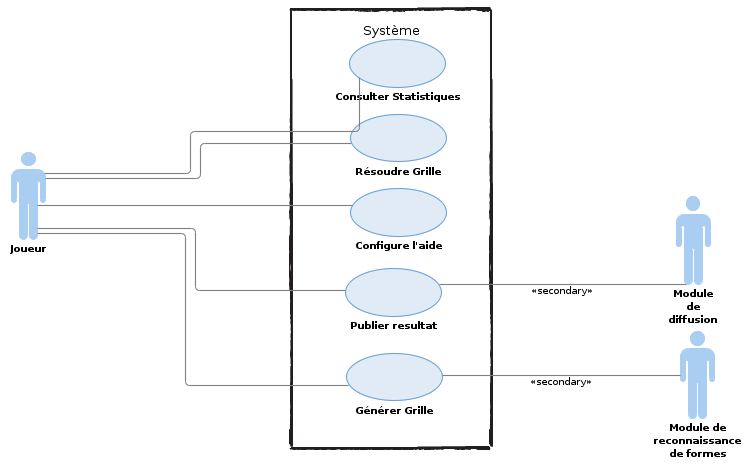
\includegraphics[scale=0.4]{diagrammeCasDUtilisation.png}
  \end{figure}
\end{frame}

\subsection{Fiches détaillées de cas d’utilisation}
\begin{frame}
  \frametitle{Fiche détaillée du cas d'utilisation « Résoudre Grille »}
  \setbeamertemplate{blocks}[default]
  \begin{block}{\footnotesize{But}}
    \scriptsize{L'utilisateur veut résoudre une nouvelle grille de sudoku}
  \end{block}
  \pause
  \begin{block}{\footnotesize{Séquencement}}
    \scriptsize{Le cas d'utilisation commence lorsque la grille apparaît sur l'écran du smartphone / tablette}
  \end{block}
  \pause
  \begin{block}{\footnotesize{Enchaînement nominal}}
    \begin{enumerate}    
      \setbeamertemplate{enumerate item}[circle]
      \item
        \scriptsize{L'utilisateur sélectionne une case vide de la grille à remplir.}
      \item
        \scriptsize{Le système affiche une aide selon le niveau de difficulté :}
        \begin{itemize}
          \setbeamertemplate{itemize item}[circle]
          \item
            \scriptsize{facile : le système affiche pour chaque case les valeurs possibles au vu du reste de la grille}
          \item
            \scriptsize{difficile : le système n'affiche rien}
        \end{itemize}
      \item
        \scriptsize{L'utilisateur entre un numéro de 1 à 9 dans cette case.}
      \item
        \scriptsize{L'utilisateur répète l'action 1 jusqu'à compléter intégralement la grille.}
      \item
        \scriptsize{L'utilisateur valide la grille.}
    \end{enumerate}
  \end{block}
\end{frame}

\begin{frame}
  \frametitle{Fiche détaillée du cas d'utilisation : « Résoudre Grille »}
  \setbeamertemplate{blocks}[default]
  \begin{block}{\footnotesize{Post-conditions}}
    \scriptsize{Le QI du joueur est mis-à-jour}
  \end{block}
  \pause
  \begin{block}{\footnotesize{Enchaînement alternatif 1}}
    \scriptsize{Le niveau est intermédiaire et l’utilisateur se trompe lorsqu’il entre une valeur dans une case. L’enchaînement démarre après le point 3) de la séquence nominale :}
    \begin{enumerate}    
      \setbeamertemplate{enumerate item}[circle]
      \item
        \scriptsize{Le système affiche un message signalant que la valeur entrée est fausse}
      \item
        \scriptsize{On retourne au point 1 de la séquence nominale}
    \end{enumerate}
  \end{block}
  \pause
  \begin{block}{\footnotesize{Enchaînement alternatif 2}}
    \scriptsize{Le niveau est difficile et la grille remplie par l’utilisateur est fausse. L’enchaînement démarre après le point 5 de la séquence nominale :}
    \begin{enumerate}    
      \setbeamertemplate{enumerate item}[circle]
    \item
      \scriptsize{Le système affiche un message signalant que la grille est fausse et remet la grille à zéro.}
    \item
      \scriptsize{On retourne au point 1 de la séquence nominale}
    \end{enumerate}
  \end{block}
  \pause
  \begin{block}{\footnotesize{Enchaînement d’Exception 1}}
    \scriptsize{On interrompt le remplissage de la grille (ou bien l’utilisateur quitte, ou bien l’application est interrompue par une application externe comme la réception d’un appel).
L’enchaînement démarre après n’importe quel point de la séquence nominale.}
  \end{block}
\end{frame}

\begin{frame}
  \frametitle{Fiche détaillée du cas d'utilisation « Configurer l’aide »}
  \setbeamertemplate{blocks}[default]
  \begin{block}{\footnotesize{But}}
    \scriptsize{Décrire les étapes de configuration de l’aide}
  \end{block}
  \pause
  \begin{block}{\footnotesize{Séquencement}}
    \scriptsize{Le cas d'utilisation démarre lorsque l'utilisateur appuie sur le bouton de configuration de l’aide.}
  \end{block}
  \pause
  \begin{block}{\footnotesize{Enchaînement nominal}}
    \begin{enumerate}    
      \setbeamertemplate{enumerate item}[circle]
      \item
        \scriptsize{Le système affiche les options d’aide}
      \item
        \scriptsize{L'utilisateur change le niveau de l’aide (facile, intermédiaire ou difficile) puis appuie sur le bouton de validation}
    \end{enumerate}
  \pause 
  \end{block}
  \begin{block}{\footnotesize{Post-conditions}}
    \scriptsize{Le système a modifié les options.}
  \pause
  \end{block}
  \begin{block}{\footnotesize{Enchaînement d’Exception 1}}
    \scriptsize{On annule la sélection des options. L'enchaînement commence après le point 1 de la séquence nominale.}
    \begin{enumerate}    
      \setbeamertemplate{enumerate item}[circle]
      \item
        \scriptsize{L’utilisateur clique sur le bouton annuler}
      \item
        \scriptsize{Le système ne modifie pas les options et laisse la configuration précédente.}
    \end{enumerate}
  \end{block}
\end{frame}

\begin{frame}
  \frametitle{Fiche détaillée du cas d'utilisation « Consulter les statistiques »}
  \setbeamertemplate{blocks}[default]
  \begin{block}{\footnotesize{But}}
    \scriptsize{Décrire les étapes de consultation des statistiques}
  \end{block}
  \pause
  \begin{block}{\footnotesize{Séquencement}}
    \scriptsize{Le cas d'utilisation démarre lorsque l'utilisateur appuie sur le bouton de consultations des statistiques}
  \end{block}
  \pause
  \begin{block}{\footnotesize{Enchaînement nominal}}
    \begin{enumerate}    
      \setbeamertemplate{enumerate item}[circle]
      \item
        \scriptsize{Le système affiche les statistiques gardées en mémoire.}
    \end{enumerate}
  \end{block}
\end{frame}
\begin{frame}
  \frametitle{Fiche détaillée du cas d'utilisation « Publier Résultats »}
  \setbeamertemplate{blocks}[default]
  \begin{block}{\footnotesize{But}}
    \scriptsize{Décrire les étapes permettant à l'utilisateur de publier ses résultats.}
  \end{block}
  \pause
  \begin{block}{\footnotesize{Séquencement}}
    \scriptsize{Le cas d'utilisation commence lorsque l'utilisateur appuie sur le bouton « Publier Résultats ».}
  \end{block}
  \pause
  \begin{block}{\footnotesize{Pre-condition}}
    \scriptsize{Le résultat doit être supérieur ou égal à 0.}
  \end{block}
  \pause
  \begin{block}{\footnotesize{Enchaînement nominal}}
    \begin{enumerate}    
      \setbeamertemplate{enumerate item}[circle]
    \item
      \scriptsize{Le système envoie aux réseaux sociaux les résultats de l'utilisateur.}
    \item
      \scriptsize{Le système indique le succès de l'envoi du résultat. }
    \end{enumerate}
  \end{block}
  \pause
  \begin{block}{\footnotesize{Enchaînement d’Exception 1}}
  \scriptsize{L'enchaînement commence après le point 1 de la séquence nominale.}
    \begin{enumerate}
      \item
        \scriptsize{Le système indique que le réseau est indisponible.}
      \item
        \scriptsize{Case se termine.}
    \end{enumerate}
  \end{block}
\end{frame}

\subsection{Diagramme de classe métier}
\begin{frame}
  \frametitle{Diagramme de classe métier}
  \begin{figure}[h]
    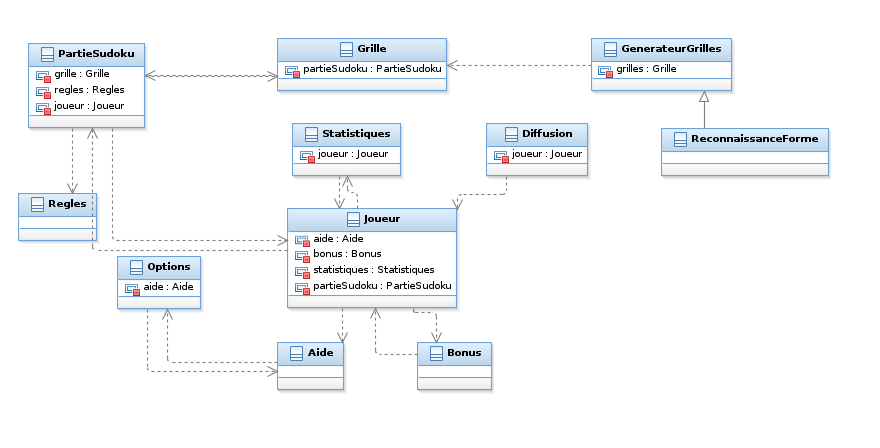
\includegraphics[scale=0.4]{diagrammeDeClasseMetier.png}
  \end{figure}
\end{frame}

\subsection{Diagramme de Séquence}
\begin{frame}
  \frametitle{Diagramme de Séquence}
  \begin{figure}[h]
    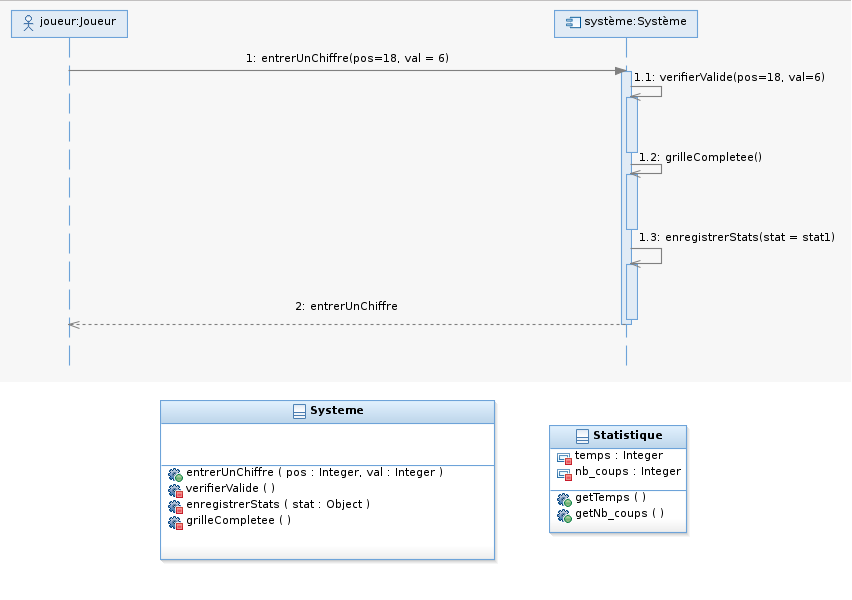
\includegraphics[scale=0.4]{LEdiagrammedesequence.png}
  \end{figure}
\end{frame}

\subsection{Tests de validation}
\begin{frame}
  \frametitle{Test de validation \no 1 du cas d'utilisation « Résoudre Grille »}
  \setbeamertemplate{blocks}[default]
  \begin{block}{\footnotesize{Titre}}
    \scriptsize{Résoudre une grille en mode facile}
  \end{block}
  \pause
  \begin{block}{\footnotesize{Contexte}}
    \scriptsize{Le niveau est mis à facile dans les options}
  \end{block}
  \pause
  \begin{block}{\footnotesize{Scénario}}
    \begin{enumerate}
      \setbeamertemplate{enumerate item}[circle]
      \item
        \scriptsize{L'utilisateur saisit un numéro dans une case vide parmi ceux proposés pour cette case}
      \item
        \scriptsize{L’utilisateur répète cette action jusqu’à compléter la grille}
      \item
        \scriptsize{L’utilisateur valide la grille}
    \end{enumerate}
  \end{block}
  \pause
  \begin{block}{\footnotesize{Résultat attendu}}
    \scriptsize{Le système affiche les statistiques de la partie}
  \end{block}
\end{frame}
\begin{frame}
  \frametitle{Test de validation \no 2 du cas d'utilisation « Résoudre Grille »}
  \setbeamertemplate{blocks}[default]
  \begin{block}{\footnotesize{Titre}}
    \scriptsize{Faire une faute en résolvant une grille en mode intermédiaire}
  \end{block}
  \pause
  \begin{block}{\footnotesize{Contexte}}
    \scriptsize{Le niveau est mis à intermédiaire dans les options}
  \end{block}
  \pause
  \begin{block}{\footnotesize{Scénario}}
    \begin{enumerate}
      \setbeamertemplate{enumerate item}[circle]
    \item
      \scriptsize{L’utilisateur saisit un mauvais numéro dans une case vide (c’est-à-dire un numéro entre 1 et 9 apparaissant déjà dans la colonne et/ou dans la ligne et/ou dans le carré).}
      \end{enumerate}
    \end{block}
    \pause
    \begin{block}{\footnotesize{Résultat attendu}}
      \scriptsize{Le système affiche un message signalant que la valeur est fausse.}
    \end{block}
  \end{frame}
  

\end{document}
